% *** Tipo de Formato del documento ***
\documentclass[journal, trans, spanish]{IEEEtran}
\usepackage[spanish, es-tabla]{babel}
\usepackage[utf8]{inputenc}
\usepackage[style=ieee]{biblatex}
\usepackage{graphicx}            % Para colocar una imagen
\usepackage{wrapfig}             % Para colocar una imagen y que a los lados haya texto
\usepackage{float}               % Para fijar una imagen después del texto, ejemplo \begin{figure}[H]
\usepackage{blindtext, english}           % Para colocar texto de prueba 

% *** Paquetería para citar referencias  ***
\bibliography{example_bib.bib}   % Para referenciar libros

% *** Paqueteria para ecuaciones matemáticas  ***
\usepackage{amsmath}             % Para editar ecuaciones matemáticas
\usepackage{newtxmath}           % Para editar el tipo de letra de las ecuaciones

% ***Paquetería para formato de Texto ***
\usepackage{url}                % Para colocar hipervínculos
\hyphenation{ho-la es-to es un e-jem-plo}  %Para separar palabras por sílabas correctamente

\begin{document}

% Titulo del Documento
\title{ Exoesqueleto para dedo índice con 6 GDL \\ \small{Reporte de Medio Término}}
\author{García Álvarez Gregorio Eliezer \\ Luna Macías Antonio de Jesús \\ Tevera Ruiz Alejandro}
        
% Encabezados
\markboth{Robótica I. Equipo 2, Octubre 2021} 
{Shell \MakeLowercase{\textit{et al.}}: Bare Demo of IEEEtran.cls for IEEE Journals}


\maketitle

\begin{abstract}
El presente documento describe el desarrollo cinemático y dinámico que simula un exoesqueleto con 6 grados de libertad (GDL). 

\noindent El diseño está enfocado para utilizarse en el dedo índice, sin embargo debido a que este trabajo aún no incorpora otras cadenas cinemáticas, como el diseño original presentado en el trabajo: "HEXOTRAC"[1], esto implica que el propio, se pueda utilizar adecuadamente en cualquier dedo a excepción del pulgar. 

\noindent Una de las características que tendrá el exoesqueleto presentado, será que el dedal distal, tendrá capacidades hápticas y estará actuado en todos sus grados de libertad, sin embargo por el momento, no es el alcance concerniente a este documento. 

\end{abstract}

\begin{IEEEkeywords}
Cinemática, Dinámica, 6 GDL, Háptica
\end{IEEEkeywords}

\section{Introducción}

\blindtext[0]

\section{Desarrollo}

\noindent El diseño del dedo exoesqueleto con 6 GDL se muestra en la Figura \ref{fig:Diseño3D} en su posición inicial de "CASA" y está constituido por una cadena cinemática de 7 eslabones, que están todos conectados entre sí por articulaciones revolutas. El software que se utilizó para generar el diseño en 3D, fue solidworks porque tiene varias herramientas que ayudaron en el desarrollo matemático, así como su versatilidad para enlazarse con matlab, software con el que se programaron los cálculos.  
\begin{figure} [H]
         \centering
         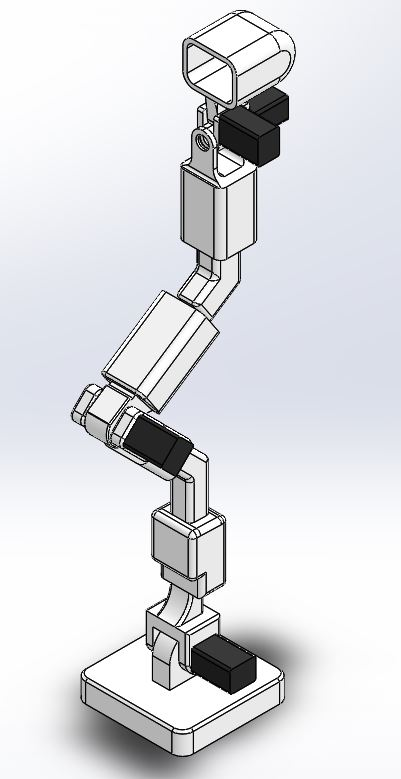
\includegraphics[scale=0.65]{Imágenes/Dedo Vist Isométrica.JPG} 
     \caption{Diseño 3D}
     \label{fig:Diseño3D}
\end{figure}
\subsection{Diseño del exoesqueleto}
\noindent La disposición de las articulaciones que se muestran en la Figura \ref{fig:EsqArtOri}, fueron las planteadas originalmente en el manual de robótica, proporcionado por el Dr. Ernesto Olguín.

\begin{figure} [H]
         \centering
         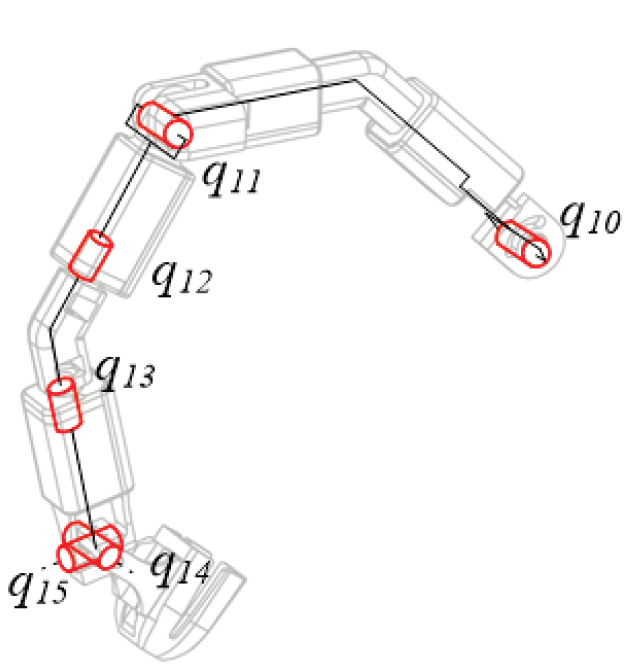
\includegraphics[scale=0.5]{Imágenes/EsquemaArticulaciones.png} 
     \caption{Esquema de las Articulaciones Original}
     \label{fig:EsqArtOri}
\end{figure}
 \noindent Sin embargo por cuestiones de practicidad el equipo propuso una modificación y se agregó un eslabón más, de esta manera se evita que la articulación revoluta  $q_1_4$ y  $q_1_5$ estuvieran fusionadas, como se visualiza en la Figura \ref{fig:EsqArtOri}. El dibujo posicionado con una perspectiva lateral derecha, que se visualiza en la Figura \ref{fig:ExoPara} proporciona una imagen con dimensiones parametrizadas, mismas que se plasman en la siguiente tabla: 

\begin{table}[!ht] %[H]
\centering
\begin{center}
\begin{tabular}{ccc}
Parámetros & [m] & [rad] \\
\hline \hline 
L1 & 0.03235525 & \\ 
L2 & 0.10513390 & \\
L3 & 0.02462267 & \\
L4 & 0.02228474 & \\
L5 & 0.04334075 & \\
L6 & 0.00600000 & \\
L7 & 0.01999013 & \\
L8 & 0.02565247 & \\
L9 & 0.01273194 & \\
L10 & 0.03641522 & \\
$\alpha$ &  & 59.26721315°\\
\end{tabular}
\end{center}
\end{table}
Así mismo, en la Figura \ref{fig:ExoPara} se aprecia la asignación de referenciales $q_1_0$, $q_1_1$, $q_1_2$, $q_1_3$, $q_1_4$, $q_1_5$, y $q_1_6$. Los marcos inerciales propuestos a cada GDL se colocaron utilizando la convención GRyMA, manteniendo la dirección positiva de la mano derecha.

También se asignaron materiales, proponiendo para los eslabones un polímero termoplástico de nombre "acrilonitrilo butadieno estireno" también conocido como filamento ABS, utilizado por impresoras 3D, pensando que en un futuro próximo podamos imprimir el modelo y así experimentar con el en un entorno real; en el caso del dedal, se seleccionó un polímero artificial que pertenece al grupo de las poliamidas, llamado comunmente "Nylon", pues creemos que para cuidar la comodidad del usuario, al ingresar su dedo, el material no debe ser tan rígido y el nylon permite un equilibrio entre la suavidad y al mismo tiempo que no sea deformable.
Finalmente los motores propuestos son de micro Metal LP con reductora de 50:1, de corriente continua, con dimensiones de 24 x 10 x 12 mm y 10 gramos de peso \\ 
\begin{figure} [h!]
         \centering
         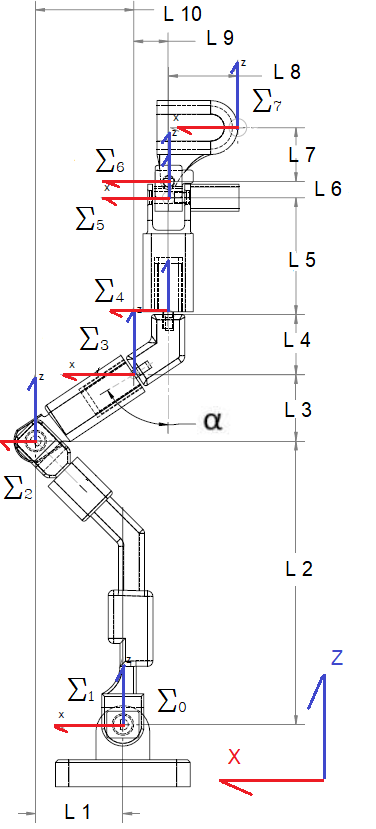
\includegraphics[scale=0.7]{Imágenes/ExoParametrizado.png}
     \caption{Esquema de las Articulaciones Utilizado}
     \label{fig:ExoPara}
\end{figure}
\noindent  \\
Conocer la cantidad de grados de libertar que tiene el exoesqueleto, nos servirá para identificar la versatilidad del movimiento que se podrá ejercer. Existen 3 clasificaciones [2] :
\begin{itemize}
    \item Menos de 6 GDL. Tienen menos GDL que el movimiento que puede tener en el espacio. Es decir, si el robot está diseñado para moverse en un espacio tridimensional (con 3 parámetros de traslación y 3 de rotación) y tiene menos de 6 GDL, presentará  limitaciones en la manera en que se mueve. 
    \item Exactamente 6 GDL. Para aquellos manipuladores robóticos que tienen exactamente 6 GDL, pueden mover su efector final de manera independiente en cada uno de los seis parámetros que conforman el espacio de trabajo tridimensional.
    \item Más de 6 GDL. Si un robot tiene más actuadores que los parámetros del espacio en el que se puede mover, implica que está sobre actuado y por lo tanto redundante.
\end{itemize}

\subsection{Cinemática directa}

\noindent La cinemática directa consiste en definir la posición y orientación del efector final, en función de las coordenadas generalizadas de cada articulación, con respescto a un marco de referencia [3], en este caso particular, es un marco de referencia no inercial.

Para lograrlo, se requieren cadenas cinemáticas desde el referencial base hasta el referencial local; para cada uno de estos ejes coordenados, se requiere el cálculo de matrices de transformación homogéneas mismas que definen el movimiento de rotación y traslación en función de donde se ubique el marco referencial de cada articulación. 

Debido a que cada eslabón tiene asignada una coordenada generalizada y por lo tanto, tiene su propia matriz que describe su movimiento, se necesita multiplicar cada una de las matrices de transformación homogéneas.
\\
La matriz de transformación homogenea tiene la siguiente forma:
\begin{equation*} A_i = 
    \begin{bmatrix}
    R^i_{i-1} & d^i_{i-1}\\
    0 & 1
    \end{bmatrix}
\end{equation*}
\noindent Cabe destacar que la matriz $R^j_i \in \mathbb{R}^{3\times 3}$ representa la orientación del referencial $j$ respecto al referencial $i$, y el vector $d^j_{i}$ expresa la traslación del referencial $j$ respecto al referencial $i$.\\

\noindent Existen diferentes métodos para asignar los referenciales de coordenadas generalizadas, y así obtener la matriz de transformación homogenea; uno de los más utilizados en robótica industrial es el denominado: "Denavit Hartenberg", pero no es el único. En el curso se presentan 2 más (Denavit Hartenberg modificado "mDH" y GRyMA), lo cierto es que los 3 buscan reducir la cantidad de parámetros que se requieren para definir las transformaciones homogéneas entre marcos referenciales. 

\noindent Los movimientos rígidos generales se definen mediante una traslación $d \in \mathbb{R}^3$ y una rotación $R \in SO(3)$. Por tanto, se componen de 6 GDL para cada par de marcos referenciales consecutivos. La asignación del marco para cada elemento rígido da como resultado todos los $A_i (q_i) \in SE(3)$ en el sistema.

\noindent Dos de los ejemplos más comunes son las convenciones clásicas de Denavit-Hartenberg (DH) y las modificadas de Denavit-Hartenberg (mDH). Ambos reducen los parámetros requeridos de 6 a 4, lo que da como resultado la torsión del enlace ($\alpha$), la longitud del enlace ($a$), el ángulo de unión ($\theta$) y el desplazamiento del enlace ($d$).
\noindent A continuación se presentarán las reglas que se deben llevar a cabo para la asignación de referenciales, correspondiente.
\\ 
\subsubsection{Denavit Hartenberg}
\\ 
\noindent Existen dos restricciones al momento de definir del marco de referencia: 
\begin{enumerate}
    \item El eje $x$ de un referencial dado debe ser perpendicular al eje $z$ de los referenciales vecinos consecutivas. 
    \item El eje $x$ de un referencial dado y el eje $z$ del referencial vecino consecutivo deben intersectar. 
\end{enumerate}

\noindent Debido a que la convención DH define una secuencia intrínseca explícita: $\theta_i \rightarrow d_i \rightarrow a_i \rightarrow \alpha_i$, las transformaciones homogéneas $A_i (q_i)$, que representan el movimiento rígido correspondiente, se obtiene la siguiente forma particular:
\begin{align*}
    A_i (q_i) & \triangleq A_R (R_{z,\theta}) A_T (d_i k) A_T (a_i i) A_R (R_{x,\alpha_i}) \\
     & = \left[  \begin{array}{cc}
        R_{i-1}^i (\cdot)  & d_{i/i-1}^{(i-1)} (\cdot) \\
         0 & 1  
\end{array} \right]
\end{align*}
donde
\begin{align*}
    R_{i-1}^i (\cdot) & = R_{z,\theta_i}  R_{x,\alpha_i} \\ 
     & = \left[  \begin{array}{ccc}
        \cos{\theta_i}  & -\sin{\theta_i}\cos{\alpha_i} & \sin{\theta_i} \sin{\alpha_i} \\
         \sin{\theta_i} &  \cos{\theta_i}\cos{\alpha_i} &
         -\cos{\theta_i}\sin{\alpha_i} \\
         0 & \sin{\alpha_i} & \cos{\alpha_i}
     \end{array} \right]
\end{align*}

\vspace{2mm}
\begin{equation*}
\begin{array}{ccc}
     d_{i/i-1}^{(i-1)} (\cdot) & = d_i k + a_i R_{z,\theta_i} R_{x,\alpha_i}  i 
     & = \left[  \begin{array}{c}
        a_i \cos{\theta_i} \\
        a_i \sin{\theta_i} \\
        d_i 
     \end{array} \right]
\end{array}
\end{equation*}

\vspace{5mm}
\noindent Además se sabe que solo uno de los parámetros DH es variable en el tiempo, por lo tanto existen variaciones en el ángulo de articulación o en el desplazamiento del enlace\\
\vspace{-2mm}
\begin{equation*}
    \begin{array}{cc}
        \theta_i (t) = \theta_{i_0} + q_i (t) & \text{Articulación Revoluta} (R) \\
        d_i (t) = d_{i_0} + q_i (t) & \text{Articulación presmática} (P)
    \end{array}
\end{equation*}
\vspace{1mm}
\noindent La cinemática directa de un robot manipulador puede ser determinada por la multiplicación de todas las matrices $A_i (q_i)$ obtenidas por la tabla de los parámetros de DH. 

\noindent Sabiendo que el exoesqueleto tiene asignados 6 coordenadas generalizadas $q_i$ se tendría que aplicar la multiplicación de la siguiente manera:
\begin{equation*}
A = A_1(q_1_0) \hspace{1mm} A_2(q_1_1) \hspace{1mm} A_3(q_1_2) \hspace{1mm} A_4(q_1_3) \hspace{1mm} A_5(q_1_4) \hspace{1mm} A_6(q_1_5) \hspace{1mm} A_7(q_1_6)
\end{equation*}
\noindent Sin embargo, esto no es del todo cierto, debido a que para lograr cumplir con las 2 condiciones que estipula la metodología, aunado a la forma que tiene el diseño de los eslabones 1 y 3, implica que se generen referenciales virtuales. 
\\ 
\noindent Después de comparar los resultados de la matriz homogenea obtenida por las 3 metodologías y comparando los resultados de las mismas, se optó por no utilizar la metodología tradicional y llevar acabo los cálculos con el siguiente método:
\\ 
\subsubsection{GRyMA}
\\ 
\noindent La metodología GRyMA (Nombre dado en honor al Grupo de Robótica y Manufactura Avanzada) es otra alternativa a la asignación de los marcos referenciales en una cadena cinemática. Busca un cambio de paradigma y no exige las restricciones de DH mencionadas en la metodología anterior. 
\\ 
\noindent El origen de cada marco de referencia $ \sum_i$ se coloca a lo largo del eje de articulación que definirá la coordenada generalizada $ qi$. No obstante, el eje z no está restringido a estar a lo largo de esta coordenada y la dirección del movimiento se define directamente con el vector director extendido $ \lambda_i=(\lambda_{Ti}^T, \lambda_{Ri}^T)^T \epsilon \thinspace \mathbb{R}^6 $. 
\\ 
\noindent Todas las coordenada generalizada de referencia, son colocadas en la misma orientación de "CASA" logrando una configuración nula y 3 parámetros de compensación son definidos para representar la distancia relativa desde el origen del marco padre para cada marco nominal $ \mathbf{d}_{io}=(d_{xi}, d_{yi}, d_{zi})$ en la posición de "CASA" (q=0).

La transformación homogenea correspondiente es $A_i$ y tiene la siguiente forma:

$A_i(qi)=A_{io}A{iV}(qi) \hfill \Sigma_i \rightarrow \Sigma_{pi},$

$A_{io}$ representa la transformación homogénea constante y $A_iv(qi)$ la transformación homogénea variante en el tiempo.
\begin{equation*}
    \hspace{-10mm}
    A_{io} = \left[
        \begin{array}{cc}
            I_{3} & d_{io}\\
            0 & 1\\
        \end{array}\right]  \epsilon \thinspace SE(3) 
\end{equation*} 

donde 

\begin{equation*}
    \hspace{-10mm}
    d_{io} = \left(
        \begin{array}{c}
            d_{xi}\\
            d_{yi}\\
            d_{zi}\\
        \end{array}\right) \epsilon \thinspace \mathbb{R}^3 
\end{equation*} 

Por otra parte:

\begin{equation*}
    \hspace{-10mm}
    A_{vi} (qi(t)) \doteq \left[
        \begin{array}{cc}
            e^{[\lambda_{Ri}X]_{qi}} & \lambda_(T_i)q_i\\
            0 & 1\\
        \end{array}\right]  
\end{equation*} 

$$ = 
\left\{\begin{matrix}
 A_R (R\lambda_{Ri,qi}) & si \thinspace qi \thinspace es \thinspace rotacional \thinspace(\lambda_T=0) \\ 
 A_T (\lambda_{Ti}qi) & si \thinspace qi \thinspace es \thinspace prismatica \thinspace(\lambda_R=0) \\ 
\end{matrix}\right.
$$
Se caracteriza con la coordenada generalizada escalar $qi\thinspace \epsilon \thinspace \mathbb{R} $ y el vector director extendido unitario constante (vector director cinemático)

$$\lambda_{i}^{(1)} {\estimates}{\overset{\scriptscriptstyle\wedge}{=}}  \begin{pmatrix} A_{Ti} \\ A_{Ri} \\ \end{pmatrix} \thinspace   \epsilon \thinspace \mathbb{R}^4 \thinspace \thinspace \Rightarrow \thinspace \thinspace \lambda_{Ti}x\lambda_{Ri}=0$$

Entonces:

$$A_{i}(q_{i})=A_{io}A_{iv}(q_{i})=\begin{bmatrix} e^{[\lambda_{Ri}X]}q_{i}& d_{io}+\lambda_{Ti}q_{i}\\ 0 & 1\end{bmatrix}$$

$e^{[\lambda_{Ri}X]qi}$ es la matriz de rotación correspondiente la cual es un mapeo exponencial (Formula de Rodrigues)

$$R_{\lambda_{i}\vartheta}=I+[\lambda x]s\vartheta+[\lambda x]^{2}\upsilon\vartheta=e^{[\lambda x]\vartheta}$$
donde
$$\upsilon_{q_{i}}= \thinspace función verseno  \thinspace\thinspace {\overset{\scriptscriptstyle\wedge}{=}} 1- cos(q_{i})$$

Si todos los movimientos posibles son alineados con uno de los ejes principales de cada marco, el vector director cinemático $\Theta_i$ se puede codificar con un parámetro escalar único i, como se muestra a continuación:

\begin{table}[!ht] %[H]
\centering
\begin{center}
\begin{tabular}{cccccccc}
$\Theta_i$ & 0 & 1 & 2 & 3 & 4 & 5 & 6\\
\hline \hline 
$\lambda_{T_i}$ & 0 & 1 & 0 & 0 & 0 & 0 & 0\\ 
$\lambda_{T_i}$ & 0 & 0 & 1 & 0 & 0 & 0 & 0\\
$\lambda_{T_i}$ & 0 & 0 & 0 & 1 & 0 & 0 & 0\\
\hline 
$\lambda_{R_i}$ & 0 & 0 & 0 & 0 & 1 & 0 & 0\\
$\lambda_{R_i}$ & 0 & 0 & 0 & 0 & 0 & 1 & 0\\
$\lambda_{R_i}$ & 0 & 0 & 0 & 0 & 0 & 0 & 1\\
\hline 
$R_{i}$ & $I_3$ & $I_3$ & $I_3$ & $I_3$ & $R_{x}(qi)$ & $R_{y}(qi)$ & $R_{z}(qi)$\\ 

\end{tabular}
\end{center}
\end{table}
En caso contrario, cada $\lambda_{T_i}$ , $\lambda_{R_i}$ puede parametrizarse con un
par elevación-azimut ($\alpha_i$, $\beta_i$):

\begin{table}[!ht] %[H]
\centering
\begin{center}
\begin{tabular}{ccc}
$\Theta_i$ & 7 & 8\\
\hline \hline 
$\lambda_{T_i}$ & $\cos{\alpha_i}\sin{\beta_i}$ & 0\\ 
$\lambda_{T_i}$ & $\sin{\alpha_i}\sin{\beta_i}$ & 0\\
$\lambda_{T_i}$ & $\cos{\beta_i}$ & 0\\
\hline 
$\lambda_{R_i}$ & 0 & $\cos{\alpha_i}\sin{\beta_i}$\\
$\lambda_{R_i}$ & 0 & $\sin{\alpha_i}\sin{\beta_i}$\\
$\lambda_{R_i}$ & 0 & $\cos{\beta_i}$\\
\hline 
$R_{i}$ & $I_3$ & $R_{\lambda_{R_i}}$ (qi)\\ 
\end{tabular}
\end{center}
\end{table}

Por lo cual, la metodología GRyMA usa únicamente 4 parámetros constantes independientes básicos  
para cada relación de los marcos padre/hijo:
$d_{xi}, d_{yi}, d_{zi}$ y $\theta$

Para la asignación de marcos se respeta el siguiente algoritmo:
\begin{enumerate}
\item Identificar los ejes de movimiento en cada articulación.
\item Asignar el marco de referencia inercial $\Sigma_0$ de modo que tanto la posición como la orientación sean estratégicamente definidas con respecto a los ejes de articulación del sistema.
\item Asignar cada marco de referencia $\Sigma_i$ a la articulación correspondiente con la misma orientación del marco inercial y con el origen a lo largo del eje de articulación.
\item Determinar el vector de distancia di0 ∈ R3 desde el marco padre de cada unión, en la posición "home" ($q = 0$).
\item Codificar el parámetro de dirección $\Theta _i$ con respecto a la dirección y el tipo de movimiento de cada articulación.
   
\end{enumerate}

\noindent Finalmente, aplicando lo anterior y asignando los marcos referenciales como se aprecia en la Figura \ref{fig:ExoPara}, se obtiene la siguiente tabla:

\begin{table}[!ht] %[H]
\centering
\begin{center}
\begin{tabular}{cccccc}
$\Sigma_i$ & $\Sigma_p_i$ & d_x_i & d_y_i & d_z_i & $\Theta_i$\\
\hline \hline 
$\Sigma_1$ & $\Sigma_0$ & 0   & 0 & 0  & 5\\ 
$\Sigma_2$ & $\Sigma_1$ & L1  & 1 & L2 & 5\\
$\Sigma_3$ & $\Sigma_2$ & -L7 & 0 & L3 & 8\\
$\Sigma_4$ & $\Sigma_3$ & -L6 & 0 & L4 & 6\\
$\Sigma_5$ & $\Sigma_4$ & 0   & 0 & L5 & 4\\
$\Sigma_6$ & $\Sigma_5$ & 0   & 0 & 0  & 5\\
$\Sigma_6$ & $\Sigma_6$ & -L8 & 0 & 0  & 0\\
\end{tabular}
\end{center}
\end{table}
\subsection{Jacobiano}
\noindent Existen dos tipos de jacobiano: El jacobiano analítico y el jacobiano geométrico. Este último depende de la configuración del manipulador y representa la relación entre las velocidades de la articulación, la velocidad lineal y angular de efector final. 
En contraparte, el jacobiana analítico es cuando el efector final se expresa con referencia a una representación mínima (ángulos de Euler) en el espacio operacional, y se calcula derivando la posición del efector final y su orientación con respecto a las variables de la articulación [6]. La matriz jacobiana de un manipulador robótico es una matriz de $6 \times N$, donde la velocidad articular $ \dot{q}$ es un vector $N$ y la velocidad espacial $v$ es un vector $-6$. La velocidad espacial y la velocidad articular están relacionadas a través de la matriz jacobiana mediante la siguiente expresión:
\vspace{-3mm}

\begin{equation*}
    \nu = J_i (q)\dot{q}
\end{equation*}
En el caso de que el manipulador tenga 6 GDL, no hay ningún problema a la hora de analizar la matriz jacobiana, ya que será una matriz de $ 6 \times  6 $ (matriz cuadrada), por lo que los cálculos de determinantes y rangos se pueden realizar sin ningún problema. Sin embargo, como se mencionó anteriormente, el diseño propuesto se clasifica como un manipulador de menos de 6 GDL. Debido a esto, la matriz jacobiana resultante será una matriz de $ 6 \times 5 $.
\vspace{2mm}
De esta manera la matriz correspondiente a jacobiana se expresa como:
\begin{equation*}
    \hspace{-10mm}
    J = \left[
        \begin{array}{ccccc}
            J_{1,1} & J_{1,2} & J_{1,3} & J_{1,4} & J_{1,5}\\
            J_{2,1} & J_{2,2} & J_{2,3} & J_{2,4} & J_{2,5}\\
            J_{3,1} & J_{3,2} & J_{3,3} & J_{3,4} & J_{3,5}\\
            J_{4,1} & J_{4,2} & J_{4,3} & J_{4,4} & J_{4,5}\\
            J_{5,1} & J_{5,2} & J_{5,3} & J_{5,4} & J_{5,5}\\
            J_{6,1} & J_{6,2} & J_{6,3} & J_{6,4} & J_{6,5}\\
        \end{array}\right] & \hspace{10mm}
\end{equation*} 
Donde los valores representados en los primeros 3 renglones, corresponden a la velocidad lineal y los siguientes 3 a la velocidad angular. 
Para el caso de la velocidad lineal, se parte de la ecuación:
\begin{equation*}
    J_{v_i} q \triangleq = \frac{\partial d_i}{\partial q}
\end{equation*}
Tomando en cuenta esto, la matriz del jacobiana de la velocidad lineal $J_{v}$ para el robot manipulador propuesto resultará de:
\begin{equation*}
     J_v = J_{v_1}(q_1) \hspace{1mm} J_{v_2}(q_2) \hspace{1mm} J_{v_3}(q_3) \hspace{1mm} J_{v_4}(q_4) \hspace{1mm} J_{v_5}(q_5)
\end{equation*}
Para el caso de la velocidad angular, se parte de la ecuación:
\begin{equation*}
    J_{\omega _i}q \triangleq = [r1_i] \times\frac{\partial r1_i}{\partial q} + [r2_i] \times\frac{\partial r2_i}{\partial q} + [r3_i] \times\frac{\partial r3_i}{\partial q}
\end{equation*}
Tomando en cuenta esto, la matriz del jacobiana de la velocidad angular $J_{\omega}$ para el robot manipulador propuesto resultará de:
\begin{equation*}
    J_\omega = J_{\omega_1}(q_1) \hspace{1mm} J_{\omega_2}(q_2) \hspace{1mm} J_{\omega_3}(q_3) \hspace{1mm} J_{\omega_4}(q_4) \hspace{1mm} J_{\omega_5}(q_5)
\end{equation*}

\subsection{Dinámica}
La dinámica estudia las causas del movimiento, esto a través del estudio de las fuerzas y torques y su efecto en el movimiento de los cuerpos (esta representada en expresiones de segundo orden). En robótica, cuando se habla de dinámica, se hace referencia a la relación existente entre el movimiento del robot y las fuerzas generalizadas sobre el. 
El modelo de Euler-Lagrange esta representado por: 
\begin{equation*}
    H(q)\ddot{q} + C(q, \dot{q}) \dot{q} + g(q) = \tau
\end{equation*}
Donde $H(q)$ es la matriz de inercia, $C(q, \dot{q})$ es la matriz de coriolis  y $g(q)$ es el vector de gravedad. De igual forma, $\tau$ es la entrada des sistema.\\ 
\subsubsection{Matriz de Inercia}
La matriz de inercia, proviene de la energía cinemática del sistema, se encuentra descrita por
\begin{equation*}
    K = \frac{1}{2} \dot{q}^T H(q)\dot{q}
\end{equation*}
De la ecuación anterior sur la matriz de inercia, expresada por
\begin{equation*}
    H(q) = \sum_{i=o} ^n \{ m_i ^0 J_{v_cm_i} ^T(q) + ^0J_{\omega_i} ^T (q) R_0 ^i(q) I_c ^i {R_0 ^i}^T (q) ^0 J_{\omega_i} (q) \}
\end{equation*}
donde $m_i$ es la masa de cada eslabón $J_{v_cm_i}^T(q)$ es la matriz jacobiana de la velocidad lineal transpuesta para el centro de masa $i$ dependiente de $q$, $J_{\omega_i} ^T (q)$ es la matriz jacobiana de la velocidad angular transpuesta de $i$  dependiente de $q$, $I_c ^i$ es la matriz del tensor de inercia de $i$ y $J_{\omega_i} (q)$ es la matriz jacobiana de la velocidad angular.
La matriz del tensor de inercia expresa el centro de masa en un marco referencial de coordenadas cartesianas. Es definida por
\begin{equation*}
    \textbf{I}_c \triangleq \int_B [r \times]^T [r \times] dm 
\end{equation*}
Dentro de las propiedades de la matriz, es que esta debe ser definida positiva. \\

\subsubsection{Matriz de Coriolis}
El vector de fuerzas centrípetas y de Coriolis están representadas por $C_{q}(q,\dot{q})\dot{q}$ 
Como la matriz de Coriolis depende del vector de coordenadas generalizadas y las velocidades correspondientes, al multiplicarla con el vector de velocidades en coordenadas generalizadas, se obtienen velocidades cruzadas (cuadrática en velocidada) y debido a ello no hay una única matriz de Coriolis. 

Calcularla con los símbolos de Christofel nos da la propiedad de anti-simetría con respecto a la matriz de inercia.

$$\left | C_{q}(q,\dot{q}) \right |{k j}=\sum_{i=1}^{n}=c_{ijk}(q)\dot{q_{i}}$$

donde: 

$$c_{ijk}(q)=\frac{1}{2}\left \{ \frac{\delta h_{kj}(q)}{\delta q_{i}}+\frac{\delta h_{ik}(q)}{\delta q_{j}}-\frac{\delta h_{ij}(q)}{\delta q_{k}} \right \}$$

El vector de Coriolis se obtiene multiplicando la matriz de Coriolis por las velocidades en coordenadas generalizadas

$$C_{q}(q,\dot{q})\dot{q}=\begin{pmatrix}
\vdots\\
\sum_{ij=1}^{n}=C_{ijk}(q)\dot{q_{i}}\dot{q_{j}}\\ 
\vdots\\
\end{pmatrix}
=\begin{pmatrix}
\vdots\\
\dot{q}^{T}C_{k}(q)\dot{q}\\ 
\vdots\\
\end{pmatrix}$$

\subsubsection{Vector de gravedad}
El vector de gravedad representa los torques sobre el robot debido al peso de cada eslabón, para obtenerlo se parte de la energía potencial. La energía potencial de cada cuerpo viene dada por su peso multiplicado por la posición vertical de su centro de masa
$$U_{i}=-m_{i}g_{0}\cdot d_{cmi}(q)=-m_{i}d^{T}_{cmi}(q)g{o'}$$
$d_{cmi}$(q) ∈ R3 es la posición cartesiana del vector de masa del cuerpo $i$

$g_0 ∈ R3$ es la expresión inercial para la dirección de la gravedad (se define de acuerdo con la definición de la referencia del marco inercial del sistema) y el signo menos es una corrección tal que la energía potencial aumenta en contra de la dirección de la gravedad.\\
La potencia total es una función que varia solo en la configuración q del sistema: 
$$g_{q}=-\sum_{i=1}^{N}m_{i}\frac{\delta d_{cmi}(q)^{T}}{\delta q}g_{0}=-\sum_{i=1}^{N}m_{i}J_{v_{cmi}}^{T}(q)g_{0}$$

donde:

$$d_{cmi}(q)=d_{i}+R^{i}_{0}(q)r_{ci}$$

La gradiente de la energía potencial es calculada como:

$$g_{q}=- \sum_{i=1}^{n}m_{i}\frac{\delta d_{cmi}(q)^{T}}{\delta q}g_{0}=-\sum_{i=1}^{n}m_{i}J_{v_{cmi}}^{T}(q)g_{0}$$

\section{Resultados}
\subsection{Jacobiana}
Como se mencionó anteriormente, la matriz jacobiana se compone de la velocidad lineal y de la velocidad angular, a fin de obtener la matriz
\begin{equation*}
    \hspace{-10mm}
    J = \left[
        \begin{array}{ccccc}
            J_{1,1} & J_{1,2} & J_{1,3} & J_{1,4} & J_{1,5}\\
            J_{2,1} & J_{2,2} & J_{2,3} & J_{2,4} & J_{2,5}\\
            J_{3,1} & J_{3,2} & J_{3,3} & J_{3,4} & J_{3,5}\\
            J_{4,1} & J_{4,2} & J_{4,3} & J_{4,4} & J_{4,5}\\
            J_{5,1} & J_{5,2} & J_{5,3} & J_{5,4} & J_{5,5}\\
            J_{6,1} & J_{6,2} & J_{6,3} & J_{6,4} & J_{6,5}\\
        \end{array}\right] & \hspace{10mm}
\end{equation*}
Como se observa la matriz obtenida es una matriz de 6 x 6, al ser una matriz cuadrada, el rango de la matriz es de 6
Para la jacobiana de la velocidad lineal se obtiene: 
\begin{equation*}
    \hspace{-10mm}
    J = \left[
        \begin{array}{ccccc}
            J_{v_1 ,1} & J_{v_1 ,2} & J_{v_1 ,3} & J_{v_1 ,4} & J_{v_1 ,5}\\
            J_{v_2 ,2} & J_{v_2 ,2} & J_{v_2 ,3} & J_{v_2 ,4} & J_{v_2 ,5}\\
            J_{v_3 ,3 } & J_{v_3,2} & J_{v_3 ,3} & J_{v_3 ,4} & J_{v_3 ,5}\\
        \end{array}\right] \hspace{10mm}
\end{equation*} 
\noindent Tomando en cuenta que cada $C_i$ corresponde a $\cos \theta_i$ y cada $S_i$ a $\sin \theta_i$, cada elemento $J_{v_ij}$ de la matriz es representado por:

 
Y para la jacobiana de la velocidad angular se tiene:
\begin{equation*}
    \hspace{-10mm}
    J = \left[
        \begin{array}{ccccc}
            J_{\omega_1 ,1} & J_{\omega1 ,2} & J_{\omega1 ,3} & J_{\omega1 ,4} & J_{\omega1 ,5}\\
            J_{\omega2 ,2} & J_{\omega2 ,2} & J_{\omega2 ,3} & J_{\omega2 ,4} & J_{\omega2 ,5}\\
            J_{\omega3 ,3 } & J_{\omega3,2} & J_{\omega3 ,3} & J_{\omega3 ,4} & J_{\omega3 ,5}\\
        \end{array}\right] 
        \hspace{10mm}
\end{equation*} 
\noindent Tomando en cuenta que cada $C_i$ corresponde a $\cos \theta_i$ y cada $S_i$ a $\sin \theta_i$, cada elemento $J_{\omegaij}$ de la matriz es representado por:
\begin{flushleft}
\(J_{\omega_1 ,1} = 0 \)\\ \vspace{0.25cm}
\(J_{\omega1 ,2} = 0\) \\ \vspace{0.25cm}
\(J_{\omega1 ,3} = 0\) \\ \vspace{0.25cm}
\(J_{\omega1 ,4} = 0\) \\ \vspace{0.25cm}
\(J_{\omega1 ,5} = 0\) \\ \vspace{0.25cm}
\end{flushleft}

\begin{flushleft}
\(J_{\omega2 ,2} = 0 \) \\ \vspace{0.25cm}
\(J_{\omega2 ,2} = 0\) \\ \vspace{0.25cm}
\(J_{\omega2 ,3} =0\) \\ \vspace{0.25cm}
\(J_{\omega2 ,4} =0\) \\ \vspace{0.25cm}
\(J_{\omega2 ,5 } =0\) \\ \vspace{0.25cm}
\end{flushleft}

\begin{flushleft}
\(J_{\omega3 ,3} = 0 \) \\ \vspace{0.25cm}
\(J_{\omega3, 2} = 0 \) \\ \vspace{0.25cm}
\(J_{\omega3 ,3} = 0 \) \\ \vspace{0.25cm}
\(J_{\omega3 ,4} = 0 \) \\ \vspace{0.25cm}
\(J_{\omega3 ,5} = 0\) \\ \vspace{0.25cm}
\end{flushleft}           




\subsection{Dinámica}
Se obtuvieron el vector de Coriolis, Inercia así como el vector de gravedad (el proceso y los resultados obtenidos se muestran más adelante). A fin de obtener la dinámica del sistema.
Cabe resaltar que para obtener las masas, los centros de masa, así como los tensores de inercia, estos fueron obtenidos del modelo CAD, los datos se describen a continuación: 
Masas:
\begin{equation*}
    M=( 0 & 0 & 0 & 0 & 0 & 0) 
\end{equation*}
Tensor de inercia: 
\begin{align*}
I_c{1} & =\begin{bmatrix}
0 &	0 &	0 \\ 0 &	0 &	0 \\
0 &	0 &	0\end{bmatrix} \\
I_c{2} & =\begin{bmatrix}
0 &	0 &	0    \\
0  &	0 &	0 \\
0	& 0 &	0\end{bmatrix} \\
I_c{3} & =\begin{bmatrix}
0 &	0	& 0 \\0	0 & 0 \\
0 & 0 & 0\end{bmatrix}\\
I_c{4} & =\begin{bmatrix}
0 &	0 & 0 \\
0 & 0 &	0\\
0 & 0 &	0\end{bmatrix}\\
I_c{5} & =\begin{bmatrix}
0 &	0 & 0\\
0 &	0 & 0\\ 
0 & 0 & 0\end{bmatrix}\\
I_c{6} & =\begin{bmatrix}
0 &	0 & 0\\
0 &	0 & 0\\ 
0 & 0 & 0\end{bmatrix}
\end{align*}
Centros de Masa 
\begin{align*}
CM_{xi}=[0 & 0 & 0 & 0 & 0 & 0]\\
CM_{yi}=[0 & 0 & 0 & 0 & 0 & 0]\\
CM_{zi}=[0 & 0 & 0 & 0 & 0 & 0]\\
\end{align*}

\subsubsection{Matriz de Inercia}
La matriz de inercia del robot manipulador esta expresada por 
\begin{equation*}
    H=\begin{bmatrix} H_{11} & H_{12} & H_{13} & H_{14} & H_15 & H_{16}\\
    H_{21} & H_{22} & H_{23} & H_{24} & H_25 & H_{26}\\
    H_{31} & H_{32} & H_{33} & H_{34} & H_35 & H_{36}\\
    H_{41} & H_{42} & H_{43} & H_{44} & H_45 & H_{46}\\
    H_{51} & H_{52} & H_{53} & H_{54} & H_55 & H_{56}\\
    H_{61} & H_{62} & H_{63} & H_{64} & H_65 & H_{66}
   \end{bmatrix}
\end{equation*}
\noindent Tomando en cuenta que cada $qi$ corresponde a $\theta_i$, $C_i$ corresponde a $\cos \theta_i$ y cada $S_i$ a $\sin \theta_i$, cada elemento $H_{ij}$ de la matriz es representado por:

\subsubsection{Vector de Coriolis}
Para el robot dedo exoesqueleto propuesto, el vector de coriolis esta expresado por:
\begin{equation*}
    C=\begin{bmatrix} C_{11}\\
                      C_{21}\\
                      C_{31}\\
                      C_{41}\\
                      C_{51}\\
                      C_{61}\end{bmatrix}
\end{equation*}
\noindent Tomando en cuenta que cada $qi$ corresponde a $\theta_i$, $dqi$ corresponde a $\dot{\theta_i}$, $C_i$ corresponde a $\cos \theta_i$ y cada $S_i$ a $\sin \theta_i$, cada elemento $C_{ij}$ de la matriz es representado por:


\subsubsection{Vector de gravedad}
El vector de gravedad final resultante de $\textbf{C}$, para el robot propuesto se representa por el siguiente vector
\begin{equation*}
    \textbf{g(q)}= \begin{bmatrix} g(q)_1_0 & g(q)_1_1 & g(q)_1_2 & g(q)_1_3 & g(q)_1_4 &g(q)_1_5 & g(q)_1_6  \end{bmatrix}
\end{equation*}
Tomando en cuenta que cada $C_1$ corresponde a $\cos \theta_i$ y cada $S_i$ a $\sin \theta_i$, cada  elemento $g(q)_i$ de vector es representado por 


\section{Discusión}

\blindtext[0]

\section{Conclusiones}

\subsection{García Álvarez Gregorio Eliezer}
\blindtext[0]
\subsection{Luna Macías Antonio de Jesús}
\blindtext[0]
\subsection{Tevera Ruiz Alejandro}
\blindtext[0]
\section{Anexos}
\blindtext[0]


\section{Referencias}
\noindent [1]    Sarakoglou, Ioannis & Brygo, Anais & Mazzanti, Dario & Garcia-Hernandez, Nadia & Caldwell, Darwin & Tsagarakis, Nikos. (2016). HEXOTRAC: A highly Under-Actuated Hand Exoskeleton for Finger Tracking and Force Feedback.. 10.1109/IROS.2016.7759176. \\
\noindent [2]    Peter Corke.Robotics, Vision and Control. Ed. by Oussama Khatib Bruno Siciliano. Springer InternationalPublishing, 2017.doi:10.1007/978-3-319-54413-7.\\
\noindent [3]    Mark Spong.Robot modeling and control. Hoboken, NJ: John Wiley & Sons, Inc, 2020.isbn: 9781119524076.\\

\end{document}


